\chapter{Microservice Architektur als Weg robuste und skalierbare Anwendungen zu entwickeln}
``Microservice Architektur'' beschreibt einen Stil der Softwareentwicklung, der vor Allem durch die Trennung einer großen Gesamtanwendung, in kleinere, separate Teile gekennzeichnet ist.~\cite[vgl.][Seite 2]{newman2015building}
Entscheidend für die Microservice Architektur ist im wesentlichen die Abgrenzung zur monolithischen Anwendungsentwicklung, ebenso wie die Abgrenzung zur Service Oriented Architecture.

\section{Microservices als Werkzeug zum Management von Komplexität}
Monolithische Anwendungen bestehen im wesentlichen aus einer einzelnen Einheit.~\cite[vgl.][]{Fowler:Intro} In einer klassischen Drei-Schichten-Anwendung (Frontend, Backend, Persistence Layer)~\cite[vgl.][]{MSDN:TTA}, wie in \autoref{fig:threetier} dargestellt, bietet es sich an, die gesamte Logik in einer Anwendung zu verwalten. Dies ist auch der Standardaufbau der meisten Webframeworks. Es gibt eine Schnittstelle zwischen der clientseitigen und der serverseitigen Anwendung, ebenso wie zwischen der serverseitigen Anwendung und der Datenbank. Unabhängig wie unübersichtlich ein System mit zunehmender Größe wird, das zusammenhalten dieser Anwendungsteile ist der Standardweg. Schwer zu handhabende, komplexe und große monolithische Anwendungen entstehen häufig dann, wenn eine Anwendung mit der Zeit wächst, der Aufbau der Anwendung jedoch nicht gut genug geplant wird.~\cite[vgl.][]{infaktuell}
\begin{figure}[!ht]
    \caption{Drei-Schichten Anwendungsverteilung (\cite{ThreeTieredDistribution})}
    \label{fig:threetier}
    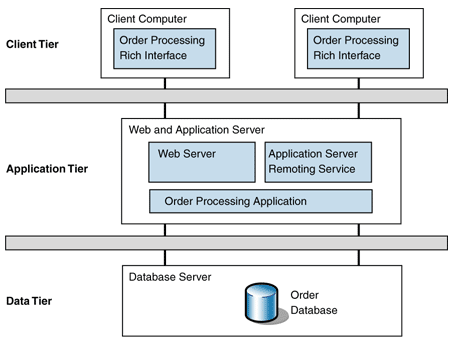
\includegraphics[width=\textwidth]{three_tier_application}
\end{figure}

Anstatt einer großen Anwendung, deren einzelne Teile gemeinsam deployt werden, in einem gemeinsamen repository liegen und auf der Ebene der genutzten Programmiersprache kommunizieren, wird bei der Microservice Architektur die Gesamtanwendung hingegen in einzelne Teilanwendungen aufgesplittet. Diese liegen in separaten Repositories, können getrennt voneinander deployt werden und kommunizieren über externe Schnittstellen. Diese separaten Teilanwendungen sind meist anhand von Aufgabengebieten getrennt und identifiziert. Die Trennung nach Single Responsibility Principle~\cite[vgl.][Seite 108]{Martin:SRP} wird hier von der Ebene des Codes in die Ebene der Gesamtarchitektur gehoben.

Ein Architekturstil, der der Microservice Architektur ähnelt, ist die ``Service-Oriented Architecture''. Aufgrund der ähnlichen Ansätze, die dieser Architekturstil verfolgt, sollte er näher betrachtet werden.
Service-Oriented Architecture (SOA) hat sich ebenfalls entwickelt, um die Probleme großer, monolithischer Anwendungen zu lösen.\cite[][Seite 8]{newman2015building} Mit Hilfe von Services, soll wiederverwendbarer Code geschaffen werden, der dann von verschiedenen Endanwendungen genutzt werden kann. Die Kommunikation findet über Netzwerke statt und nicht mehr über direkte Aufrufe im Code. Auch SOA soll es einfacher machen Code zu organisieren, zu strukturieren und bei Bedarf zu ersetzen. Warum entsteht nun also der Trend der Microservices, wenn SOA einen ähnlichen Ansatz verfolgt? Ein großes Problem von SOA liegt eigentlich in den damit verbundenen Technologien wie SOAP, vendor middleware und der nicht ausreichend klaren Trennung der Services.\cite[][Seite 8]{newman2015building} 
Ein weiterer Unterschied zwischen SOA und Microservice Architektur ist grundsätzlich auch die Kommunikation zwischen den Services. Wo SOA häufig zu komplexer Logik mit dem Enterprise Service Bus\cite[][]{esb} tendiert, setzt die Microservice Architektur Gemeinschaft gemeinhin auf das an das Unix Prinzip der ''Pipes and Filters''\cite[vgl.][]{microsoft:pipes} angelehnte Prinzip der ''Smart Endpoints und Dumb Pipes''.\cite[vgl.][]{Fowler:Intro}
SOA scheint im Allgemeinen nicht klar genug definiert zu sein.~\cite[vgl.][]{Fowler:Intro} Daher ist es ratsam einen klarer definierten Begriff, wie den der Microserice Architektur anzustreben,\cite[][]{Fowler:Intro} dies heißt jedoch nicht zwangsläufig eine Abgrenzung zu allem was SOA ist. SOA verfolgt ähnliche Ansätze und ist ein entscheidender Teil der Geschichte der Microservice Architektur.

Einige der Probleme monolithischer Anwendungen lassen sich durch die Aufteilung in Services lösen oder verbessern. Microservice Architektur birgt jedoch seine ganz eigenen Herausforderungen. Microservice Architektur bringt demnach vor allem Unterschiede mit sich. Die Frage ob sich diese positiv oder negativ auswirken, hängt ganz individuell von der bestehenden Anwendung, dem Entwicklerteam und den vorhandenen Ressourcen ab.

\section{Herausforderungen und Potentiale von Microservices}
Wie bei jedem Architekturstil, gibt es sowohl Vorzüge, als auch Nachteile der Microservice Architektur.~\cite[vgl.][]{Fowler:Guide}
Bei der Entscheidung ob Microservices im Unternehmen eingesetzt werden sollten, müssen diese Vor- und Nachteile der Microservice Architektur abgewogen werden.
Im folgenden werde ich die Vor- und Nachteile des Architekturstils auf den verschiedenen Ebenen der Struktur des Codes, Technologieheterogenität, Systemverteilung, Testing, Deployment, Skalierbarkeit und Entwicklungszeit erläutern.

\subsection{Struktur des Codes}
Microservice Architektur verspricht zum einen klarere Strukturen. Seperate, nach Aufgabengebiet unterteilte Services führen zu klar strukturierten Codebases. Diese aufgeteilten Codebases verschaffen einen besseren Überblick, sodass sich Entwickler leichter in ein Aufgabe einarbeiten können ohne sich durch irrelevante Codeteile arbeiten zu müssen. Gerade in größeren Teams ist dies von großem Vorteil. Je mehr parallel an voneinander abhängigen Codeteilen gearbeitet wird, desto mehr merge Konflikte entstehen. Auch wenn die eigentlichen Aufgaben komplett voneinander getrennt sind, kommt es häufig zu Konflikten. Je vermischter der Code ist, desto mehr Konflitke enstehen. Ähnlich wie das Single Responsibility Principle auf Methoden- oder Klassenebene gilt, so kann man es auch auf Service Ebene als geltend ansehen. Getrennte, klar strukturierte Codeteile erhöhen die Wiederverwendbarkeit, erleichtern die Einarbeitung und das Management des Codes. Ebenso können Änderungen leichter eingearbeitet werden, da die Chance von Seiteneffekten reduziert ist. Komplexitäten werden demnach nicht per sé reduziert, sie werden jedoch aufgetrennt und verschoben. Somit werden sie leichter zu handhaben.

Interessant ist es hier auch auf die Teamstruktur einzugehen. Conway's Law\cite{conwayslaw} deutet hier darauf hin, dass die Struktur von Teams, sich direkt auf die Struktur von entwickelten Systemen auswirkt. Demnach ist es durchaus eine Herausforderungen klare Strukturen zu schaffen, wenn es nur ein Entwicklungsteam gibt. Die bewusste Entwicklung von separaten Services, denen ggf. bestimmte Entwickler zugewiesen werden, ist demnach ratsam um klare Strukturen zu schaffen. Ein Team und eine Codebase mit unklaren Aufgabenbereichen führt hier scheinbar fast zwangsläufig zu vermischten Strukturen im Code.
%(FIX TODO CONWAYS LAW)

So lassen sich zum Einen kleinere, autonome Anwendungsteile aus Entwicklersicht besser verwalten. Die einzelnen Anwendungsteile müssen jedoch über eine externe Schnittstelle kommunizieren. Diese Aufrufe, die in der Regel über das Intra- oder Internet stattfinden sind aufwändiger als simple Code Calls. Wie diese API Aufrufe stattfinden ist nicht zwangsläufig vorgeschrieben. Im Allgemeinen gilt jedoch: Verteilte Systeme sind schwieriger zu programmieren, da remote calls langsam und fehleranfälliger sind.~\cite[vgl.][]{Fowler:Guide}

\subsection{Technologieheterogenität}
Separate Services ermöglichen auch, komplett verschiedene Technologiestacks einzusetzen. Im Gegensatz zur Erweiterung einer monolithischen Anwendung, muss hier theoretisch nur bedingt auf die bereits eingesetzten Technologien geachtet werden. Ein separater Service mit separater Datenbank kann durchaus eine andere Datenbanktechnologie verwenden. Da über den separaten Service ohnehin ein separates Datenbankadapter implementiert werden muss, ist es aus reiner Implementierungssicht nicht nachteilig eine andere Datenbanktechnologie zu wählen. Hierbei kann durchaus auf die für den Anwendungsfall spezifischen Optimierungsmöglichkeiten geachtet werden. Ebenso kann eine für den Anwendungsfall optimierte Programmiersprache gewählt werden.
Das diese verschiedenartige Technologiewahl aus technischer Sicht möglich und ratsam ist, heißt jedoch keineswegs, dass sie tatsächlich so gewählt werden sollte. Die bestehenden Technologien in einem Unternehmen, welches beschließt eine große, bestehende Anwendung in Microservices aufzuteilen oder um einen Microservice zu erweitern, sind in der Regel tried and tested. Eine Vielzahl der Entwickler des Unternehmens wird mit den bestehenden Technologien vertraut sein. Fällt ein Entwickler aus, sind vermutlich noch genug andere Entwickler mit ähnlichen Fähigkeiten vorhanden um in dringenden Fällen die Arbeit zu übernehmen. Wählt man nun aber eine neue Programmiersprache, eine neue Datenbanktechnologie und neue Monitoring Tools aus, so ist dies ggf. nicht nur mit erhöhter Einarbeitungszeit verbunden, sondern auch mit höheren Managementkosten. Müssen neu eingstellte Entwickler nun den gesamten Technologiestack beherrschen oder nur einen der zwei Teile? Sind immer ausreichend Entwickler vorhanden um einen ausfallenden Entwickler zu kompensieren? Was passiert wenn der Entwickler des neuen Go Microservices kündigt und kein anderer Entwickler Go beherrscht? Die technologische Heterogenität kommt demnach zu einem Preis. Man sollte genau abwägen, bis zu welchem Grad die Diversifizierung des Technologiestacks lohnenswert ist.~\cite[vgl.][Seiten 5, 6]{newman2015building}
Die Definition eines klaren, ``erforderten Standards''~\cite[vgl.][Seiten 20, 21]{newman2015building} bietet sich hierzu an. Twitter und Netflix limitieren hierzu z.B. auf Technologien die unter der Java Virtual Machine (JVM) betrieben werden können.~\cite[][Seite 6]{newman2015building} Entwickler können so eine neue Programmiersprache wie Scala oder JRuby wählen, es wird jedoch auf bekannte Technologien im Betrieb des Servers gesetzt. Dieser erforderte Standard bezieht sich auch auf die gewählten Wekzeuge zum Monitoring und die eingesetzten Schnittstellentechnologien.~\cite[vgl.][Seite 21]{newman2015building} So sollte nicht jeder Microservice ein anderes Montoring Tool verwenden und die Clientanwendung nicht zu jedem Microservice eine andere Schnittstellentechnologie einbinden.

\subsection{Verteilte Systeme}
Eine große Herausforderung bei der Verwendung von Microservice Architektur, ist vor allem auch die Tatsache das es sich schlichtweg um verteilte Systeme handelt.~\cite[][]{microtradeoffs}
Tanenbaum und Van Steen definieren Verteilte Systeme als Sammlung unabhängiger Computer, die zum Benutzer als eine einzige, kohärente Einheit erscheinen.~\cite[][Seite 2]{tanenbaum2002distributed}
Zwar haben wir klar getrennte Systeme, die von der Codebase her gut zu managen sind, remote calls sind aber immer fehlerbehaftet. Der Service kann über das Netzwerk unerreichbar sein, die Antwort zu lange dauern und zu einem Timeout führen und im Allgemeinen dauern remote calls länger als code calls. Timeouts und langsame Serviceantworten können natürlich über asynchrone Aufrufe umgangen werden, aber asynchrone Aufrufe bringen ihre eigenen Probleme mit sich. Nicht umsonst spricht man hier oft in der Entwicklung von der Callback-Hell.~\cite[vgl.][]{callbackhell} Zweifelsohne kann die Callback-Hell vermieden werden, die Integration einer Netzwerkschnittstelle in die Codebase birgt aber immer Gefahren. Man kann schlichtweg nicht von einem sicheren Netztwerk ausgehen, demnach bedarf es einem Sicherheitsmechanismus zur Authentifizierung. Bandbreite kann ggf. mit Kosten verbunden sein und ist nicht unbegrenzt verfügbar sein. Außerdem kann das Netztwerk unzuverlässig sein.~\cite[vgl.][]{distributedfallacies}

Zudem müssen separate Systeme auch einzeln überwacht werden. Wo monolithische Anwendungen eine Quelle von Metriken, eine Anwendung zu überwachen und eine Anwendung zu deployen haben, haben Microservices viele.~\cite[vgl.][]{Heroku:GoMicro}

\subsection{Testing}
\label{section:testing}
In diesem Zug sollte auch das Thema Testing angesprochen werden. Testen, gerade über die Grenzen von Services hinweg, ist durchaus eine ganz eigene Herausforderung. Auf der anderen Seite haben große monolitische Anwendungen oftmals eine lange Testlaufzeit. Ab einer gewissen Größe ist es kaum noch möglich, dass der Entwickler alle Tests lokal ausführt. Der Einsatz von Continuous Integration (CI) schafft hier natürlich Abhilfe, doch auch hier sind die Ressourcen nicht unbegrenzt. Bei einer Vielzahl von Entwicklern, die parallel arbeiten, können auch mit mehreren concurrent builds Buildstaus oft nicht vermieden werden. Separate Codebases mit separaten kleineren Tests, haben hier vor Allem den großen Vorteil, dass nicht alle Tests immer erneut ausgeführt werden müssen. Bei reinen Unit Tests kann so mitunter viel Zeit gespart werden.

Eine große Herausforderung beim Einsatz von Microservices ist jedoch das Testen selbst. Treten im Live Betrieb Fehler auf, ist es nicht leicht herauszufinden wo der Fehler wirklich entsteht. Ist es ein Fehler im konsumierten Service, im konsumierenden Service oder in der Kommunikation zwischen den beiden Seiten?

\begin{wrapfigure}{l}{0.5\textwidth}
    \caption{Das Testing Board zum Testen mit Microservices \cite{rails:soa}}
    \label{fig:testboard}
    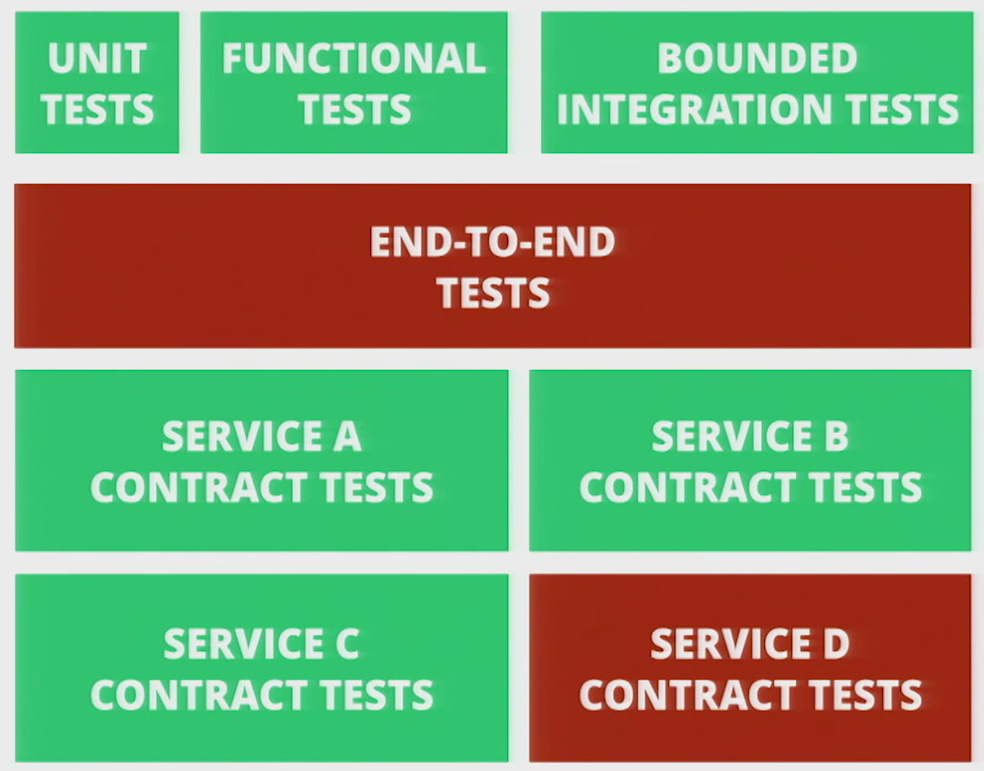
\includegraphics[width=0.5\textwidth]{testing_board}
\end{wrapfigure}

Hierzu bietet es sich an verschiedene Testebenen einzuführen. Zum Einen sollten natürlich immer sowohl der Client, als auch der Server selbst voll getestet sein. Als Weiterführung dessen, bieten sich sogenannte ``Bounded Integration Tests''\cite[vgl.][]{rails:soa} an. Bounded Integration Tests mocken im Endeffekt konsumierten Services. Dies kann zum Einen in-process geschehen, zum Anderen out-of-process. Beim in-service Mocking wird vorgegeben, die Anwendung würde mit einem externen Service sprechen, in Wahrheit geschieht jedoch gar keine Kommunikation nach Außen. Es wird angenommen, dass der Service auf eine bestimmte Anfrage in einer bestimmten Weise antwortet, dies wird entsprechend gemockt. Beim out-of-process Mocking wird ein Pseudoservice erstellt. Dieser antwortet auf bestimmte Requests so wie es vom Service erwartet wird. Es findet also eine Kommunikation nach Außen statt, jedoch nicht mit dem echten Service. Hier testen wir unsere Handhabung der erwarteten Antworten des konsumierten Services, beim out-of-process Mocking testen wir weiterhin auch die Netzwerkkonfiguration unseren Microservices.\cite{fowler:mstesting}
Als Erweiterung der Bounded Integration Tests, die den eigenen Service und die abgeschickten Abfragen testet, bieten sich Contract Tests an.~\cite[vgl.][]{fowler:contracts} Contract Tests testen den konsumierten Service, indem Sie Anfragen verschicken und die zurückgelieferten Antworten überprüfen. Hier testen wir also den Bounded Context~\cite[vgl.][]{fowler:bounded} des konsumierten Services und die Kommunikation mit ihm. Außerdem wird hier aber auch das Verständnis vom Service selbst überprüft, es muss schließlich nicht zwangsläufig der Service fehlerhaft sein, es kann auch das Verständnis des Services oder schlichtweg dessen Dokumentation fehlerhaft sein.
Bounded Integration Tests und Contract Tests, ergänzt durch \textit{End-to-End} Tests bilden mit den üblichen Unit und Integration Tests der Einzelanwendungen einen guten Test Stack, der die Fehlerfindung erheblich erleichtert. So würde ein einfacher Fehler im Betrieb der in \autoref{fig:testboard} dargestellten Anwendung ohne diese komplexen Tests schwer nachzuvollziehen sein. Mit Hilfe des Einsatzes aller Tests auf dem Test Board, kann die genaue Fehlerquelle jedoch leicht identifiziert werden.

All diese Tests lassen die Testkomplexität jedoch schnell stark ansteigen. Wenn verschiedene Mock Services gestartet, asynchrone Services getestet werden müssen und generell viele \textit{moving Parts} im System zusammen kommen, kommt es leicht zu einem Anstieg der Fehlerrate, der Testlaufzeit und der Wartungskosten.\cite{fowler:mstesting} Daher sollten nicht zu viele \textit{End-to-End} Tests geschrieben werden. Der Sinn und Zweck ist hier schließlich nicht noch einmal jedes System zu testen, sondern lediglich das Zusammenspiel aller Teile.

Interessant beim Testen von verteilten Systemen, sind hier auch Ansätze wie ``Failure Injection Testing''.\cite[][]{netflix:fit} Hier werden Systemfehler bewusst und kontrolliert auf kleiner Skala provoziert und dann das Verhalten des Gesamtsystems beobachtet. Konkret ist hier z.B. Netflix's Chaos Monkey\cite[][]{netflix:chaosmonkey} zu nennen. Alle Dienste von Netflix werden auf Amazon Web Storage (AWS)\cite{aws} betrieben. AWS Bietet hier Auto Scaling Groups (ASG). Je nach Last werden neue Serverinstanzen innerhalb festgelegter Regeln hochgefahren um die Last auf den Services angemessen zu handhaben. Der Chaos Monkey fährt nun auf einer bestimmten ASG randomisiert Instanzen herunter. Nach den Regeln der ASG sollte nun eine neue Instanz hochgefahren werden um die Alte zu ersetzen. Das System sollte nun eine messbare, aber keine relevante Verschlechterung der Antwortzeiten des Services erfahren. Interessant ist hier, wie gut das System mit dem Ausfall umgeht, wie schnell das System wieder die volle Leistung hat (mean time to recovery) und ob ggf. durch das Zusammenspiel von Services größere Fehler zustande kommen als erwartet. Aufgrund des kleinen, kontrollierten Ausfalls, ist die Wahrscheinlichkeit allzu großer Auswirkungen, selbst bei unerwarteten Fehlern, gering. Die Erkenntnisse des Failure Injection Testings können jedoch wertvoll sein und größere Probleme bei umfangreicheren Ausfällen vermeiden. Netflix selbst bewertet diese Testmethode als vollen Erfolg und weitete Failure Injection Testing vom Chaos Monkey auf weitere Testgebiete aus. So finden sich heute fünf weitere Monkeys und der Chaos Gorilla im aktiven Einsatz.\cite[][]{netflix:army}.

Ein weiterer Ansatz, der unter das Testen im Produktionsbetrieb fällt, sind graduelle bzw. staged Rollouts. Hier wird eine neuer Dienst nur für einen bestimmten Teil der Anfragen freigeschaltet. In der Regel wird hier einfach mit Hilfe eines dem Load Balancing ähnlichen Systems prozentual immer mehr der Anfragen auf den neuen Dienst geleitet. Gleichzeitig wird die Rate und die Art der auftretenden Fehler beobachtet. Steigt die Fehlerrate mit zunehmender Umleitung der Anfragen oder treten neue Fehler auf, kann dies in der Regel auf den neuen Dienst zurückgeführt werden. Ein ähnliches System nutzt Google zum Beispiel beim Veröffentlichen neuer Android Versionen.\cite[vgl.][]{Google:staged}

All diese Ansätze ersetzen natürlich keineswegs das klassische Testen vor der Veröffentlichung von Software. Sie bieten sich aber als ergänzende Testmethoden an um vor Allem die wachsende Komplexität von Softwaresystemen zu testen.

\subsection{Deployment}
Die Aufteilung einer einzelnen Codebase, die zusammen deployt wird, in mehrere Codebases bringt zwingend ebenfalls Änderungen mit sich.
Zum Einen können relativ kleine Änderungen leichter deployt werden, da nicht das gesamte System erneut deployt werden muss. Bei großen, komplexen Anwendungen können diese großen deploys ein nicht zu vernachlässigendes Risiko bilden. Und ist das Deployment einer Anwendung risikoreich, wird im Allgemeinen seltener deployt. Features werden erst später deployt, doch mit wachsenden Unterschieden zwischen Deployments, wächst auch das Risiko von Fehlern.~\cite[vgl.][Seite 6]{newman2015building}
Separate Deploys von Microservices machen die Versionierung von diesen jedoch um so wichtiger~\cite[vgl.][Seite 62]{newman2015building}$^,$~\cite[vgl.][]{Vergleichsartikel}. Breaking Changes können nicht einfach deployt werden und da gleichzeitige Deploys verschiedener, mit einander kommunizierender Services nicht möglich sind, müssen diese Deploys schrittweise und kontrolliert durchgeführt werden: Zunächst muss der Service um eine neue Version erweitert werden, die alte Schnittstelle darf hierbei nicht verändert werden. Meist werden hierzu API Versionen genutzt. So kann die erste Schnittstelle über die URL

\begin{lstlisting}[language=Ruby]
https://meinservice.tld/api/v1/eineRoute
\end{lstlisting}

\noindent angesprochen werden. Diese Schnittstelle wird von den Änderungen nicht tangiert. Die neue Schnittstelle umfasst sowohl die neuen, als auch alle alten, weiterhin gewünschten, Funktionen. Sie ist über die URL

\begin{lstlisting}[language=Ruby]
https://meinservice.tld/api/v2/eineRoute
\end{lstlisting}

\noindent anzusprechen. Nach Deploy dieser neuen Service Version, wird als nächstes der konsumierende Code geupdated. Hierbei wird die Nutzung der Funktionen auf die neue Version aktualisiert und die Request auf die neue URL umgeleitet. Alle Referenzen zur alten Route des konsumierten Services sollten hierbei entfernt werden. Abschließend kann, solange sichergestellt ist, dass die alte Service Version nicht mehr genutzt wird, der Service ein weiteres mal geupdated werden. Hierbei wird der Code der alten Version entfernt. Dies ist in der Regel nur bei firmeninternen APIs üblich. Externe APIs sollten in veralteten Versionen noch eine gewisse Zeit angeboten werden. Sollte in der neuen API Version ein Fehler auftreten, muss, vorausgesetzt v1 ist unverändert zu erreichen, nur der konsumierende Service gerollbacked werden.
Datenbankmigrationen müssen hier nach dem gleichen Prinzip ebenso in mehreren Schritten durchgeführt werden.
Versionierung ist vor Allem bei APIs mit externen Konsumenten, wie Clientanwendungen, da Updates hier nicht sofot geschehen und nicht kontrolliert werden kann, ob noch alte Routen aufgerufen werden. Bei reinen browserseitigen Clientanwendungen Anwendungen ist die Versionierung nicht zwingend notwendig, kann aber dennoch nützlich sein.
Das deployment kann also in vielen Fällen bei Microservices leichter sein, gestaltet sich bei großen Änderungen jedoch schwieriger.

\subsection{Skalierbarkeit}
Ein weiterer interessanter Punkt zum Betrieb von Microservices, ist das Thema der Skalierbarkeit.
Das ``Scale Cube''\cite[][]{abbott2009art} Modell beschreibt die drei Dimensionsen der Anwendungsskalierbarkeit. Klassische Anwendungsskalierung geschieht vor allem auf der X-Achse, der horizontalen Duplikation\cite[][]{abbott2009art}. Skaliert wird hier, indem eine Anwendung dupliziert wird. Ein Load Balancer verteilt dann, nach bestimmten Regeln, die ankommenden Requests auf verschiedene Server.~\cite[vgl.][]{loadbalancing} 

\begin{figure}[!ht]
    \caption{Die Dimension des Skalierens (\cite{abbott2009art})}
    \label{fig:scalecube}
    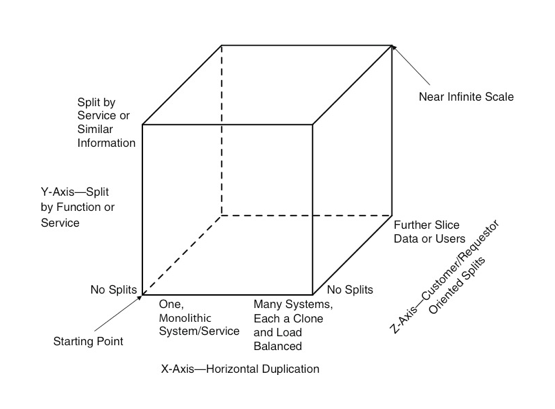
\includegraphics[width=\textwidth]{scale_cube}
\end{figure}

Die Skalierung monolithischer Anwendungen beschränkt sich in der Regel insbesondere auf dieses Load Balancing.~\cite[vgl.][]{infaktuell} 
Da die Anwendungsreplikationen funktional identisch sind, ist die verteilte Last unabhängig von den einzelnen Anwendungsteilen. Diese können eine unterschiedliche Individuallast haben, dies kann jedoch über den Load Balancer nicht beachtet werden.

Bei Microservices kann nun weiterhin auf der Y-Achse skaliert werden. Hier handelt es sich um eine funktionale Dekomposition.~\cite[][]{abbott2009art} Anwendungen werden hier in verschiedene Services unterteilt. Jeder Service ist für eine bestimmte Funktion zuständig. So kann weitaus granulärer skaliert werden. Erfährt ein Teilsystem besonders viel Last, kann dieses beliebig skaliert werden. Die anderen Teilsysteme bleiben davon unberührt. Dies optimiert sowohl Leistung, als auch Kosten.

Zusätzlich können sowohl monolithische Anwendungen, als auch Microservice auf der Z-Achse skaliert werden. Hier handelt es sich vor Allem um Datenpartionierung. So werden Datenbanksysteme oft gesharded.\cite[][]{microsoft:sharding} Dieses Sharding trennt Daten die eigentlich zusammengehören. Anhand bestimmter Kriterien werden Rows einer Datenbank auf verschiedene Systeme verteilt. Diese Partitionen bilden sogenannte Shards und können z.B. auf verschiedene Datenabankserver verteilt werden.

\subsection{Entwicklungszeit}
Zu guter Letzt sollte man die reine Entwicklungszeit betrachten. Zwar ist die separate Codebase im Nachhinein ggf. leichter zu verwalten, die initiale Entwicklung ist aber durchaus mit einem gewissen Mehraufwand verbunden. Die Wahl der optimalen Technologien ist mit Recherche verbunden, der Einsatz neue Technologien darüber hinaus mit einer Einarbeitungszeit. Das initiale Setup von Programmiersprache, Framework und Datenbank ist ein zusätzlicher Aufwand, der bei der Erweiterung einer bestehenden Codebase nicht anfällt. Hinzu kommt außerdem die Einrichtung des Deployments. Git, CI / Contiuous Deployment, Servereinrichtung, sowie das Monitoren und Warten der Server sind vor allem zum Beginn des Lebenszyklus eines neuen Microservices ein nicht unerheblicher Mehraufwand. Dies und andere Herausforderungen gegen die Potentiale der Microservice Architektur abzuwägen, muss im konkreten Einzelfall immer individuell geschehen.

\section{Der Weg zum Microservice}
Zwar scheinen Microservices ein grundsätzlich lohnenswerter Architekturstil zu sein, die Frage des Einsatzgebietes und der Umsetzung stellt sich dennoch. Fowler argumentiert\cite[][]{fowler:monolithfirst}, erfolgreiche Microservice Architekturen entstehen im Allgemeinen meist aus monolithischen Anwendungen, nicht aber, wenn von Anfang an der Einsatz von Microservices gewählt wird. Dies scheint vor Allem zweierlei Gründe zu haben: Zum Einen ist der relative Erfolg von Anwendungen grundsätzlich relativ gering. Die monolithische Anwendungsentwicklung ist nun zu Beginn schneller und einfacher und erlaubt so eine höhere Agilität. Dies erlaubt es leichter und schneller Anpassungen in jungen Anwendungen vorzunehmen um anfängliche Probleme zu lösen. Die komplexere Microservice Architektur bietet in dieser Anfangsphase keine Vorteile. Zum Anderen ist am zu Beginn des Lebenszyklus einer Anwendung schlichtweg nicht klar, um welche Aufgabengebiete sie mit der Zeit wachsen wird. Es ist nicht klar welche Teile der Anwendung besonders wichtig sein werden und welche Anwendungsteile mit der Zeit obsolet werden. Eine monolithische Anwendung erlaubt hier zunächst mehr Dynamik.

\begin{figure}[!ht]
    \caption{Produktivität nach Komplexität: Monolith und Microservices \cite{fowler:micropremium}}
    \centering
    \label{fig:micrpremium}
    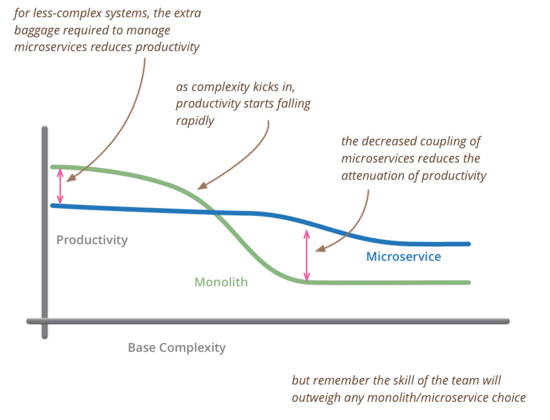
\includegraphics[width=0.8\textwidth]{micropremium}
\end{figure}

Die Aufteilung von monolithischen Anwendungen in Micrsoservices wird jedoch weitaus leichter, wenn die Struktur der Teilgebiete von Monolithen klar definiert ist. Bei der Aufsplittung des Monolithen bietet es sich hierbei an, sich am Saum (engl. seams) zu orientieren. Feathers definiert seams als ``a place where you can alter behavior in your program without editing in that place''.\cite[][Seite 29]{feathers2004working} Wir haben hier also eine klare Trennung zwischen zwei Codeteilen. So kann es sich hier z.B. um eine Objektinstanziierung handeln. Wenn die Funktion des Objektes verändert werden kann, ohne das der Aufruf der Methoden des Objektes verändert wird und außerdem kein anderer Code in seiner Funktion beeinträchtigt wird, dann sprechen wir von Seams. Codeteile, die isoliert sind und ohne Seiteneffekte geändert werden können, eignen sich besonders gut um in separate Services verschoben zu werden. Natürlich ist es alles eine Frage der konkreten Problematik, ob ein Service frei, neu gewählt werden kann oder aus Notwendigkeit, unabhängig vom Grad der Komplexität, geschaffen werden muss. Solche klaren Grenzen können bewusst in der Entwicklung von Monolithen geschaffen werden und erleichtern die Aufsplittung in separate Services enorm.

Weiterhin stellt sich die Frage wie der Microservice in Betrieb genommen wird. Bildet der Microservice ein neues Feature, kann er schlicht eingebunden werden. Ersetzt der neue Service jedoch einen bestehenden Anwendungsteil, sollte hier mitunter nicht sofort die Anwendung umgestellt werden. Wie in \autoref{section:testing} beschrieben, bietet es sich an hier nach einem dem Load Balancing ähnlichen System nach und nach mehr Last auf den neuen Anwendungsteil zu leiten und das Fehlerverhalten zu überwachen.

Ein Ansatz zum allgemeinen Ersetzen alten Codes durch neuen, ist das Strangler Pattern\cite[][]{Fowler:Strangler}. Hier wird im Live Betrieb immer mehr Code an sich eignenden Stellen ersetzt und parallel betrieben. Eine neue Anwendung kann hier in agiler Weise um den bestehenden Code gewoben werden und diesen Schlussendlich komplett ersetzen.
%(FIX Strangler Pattern hier nur angerissen, Dopplung. hmmm)